%File: formatting-instruction.tex
\documentclass[letterpaper]{article}
\usepackage{aaai}
\usepackage{times}
\usepackage{helvet}
\usepackage{courier}
\usepackage{amsmath}
\usepackage{comment}
\usepackage{amssymb}
\usepackage{amsfonts}
\usepackage{algorithm}
\usepackage{algorithmicx}
\usepackage{algpseudocode}
\usepackage{amsthm}
\usepackage{natbib}
\usepackage{textcomp}
\usepackage{graphicx}
\usepackage{multirow}

\theoremstyle{plain} \newtheorem{theorem}{Theorem} \newtheorem{proposition}{Proposition} \newtheorem{lemma}{Lemma}
\newtheorem*{corollary}{Corollary}  \newtheorem{claim}{Claim} 

\theoremstyle{definition} \newtheorem{definition}{Definition} \newtheorem{conjecture}{Conjecture} \newtheorem*{example}{Example} 

\theoremstyle{remark} \newtheorem*{remark}{Remark} \newtheorem*{note}{Note} \newtheorem{case}{Case}

\newcommand{\R}{\mathbb{R}}
\newcommand{\Astar}{A$^*$}

\frenchspacing
\pdfinfo{
/Title (Faster Optimal Planning with Partial-Order Pruning)
/Subject (AAAI Publications)
/Author (Redacted)}
\setcounter{secnumdepth}{0}  
 \begin{document}
% The file aaai.sty is the style file for AAAI Press 
% proceedings, working notes, and technical reports.
%
\title{Faster Optimal Planning with Partial-Order Pruning}
%%\author{AAAI Press\\
%Association for the Advancement of Artificial Intelligence\\
%2275 East Bayshore Road, Suite 160\\
%Palo Alto, California 94303\\
%}
\author{}

\maketitle
\begin{abstract}
\begin{quote}
  When planning problems have many kinds of resources or high
  concurrency, each optimal state has exponentially many minor
  variants, some of which are ``better" than others. Standard methods
  like \Astar cannot effectively exploit these minor relative differences,
  and therefore must explore many redundant, clearly suboptimal
  plans. We describe a new optimal search algorithm for planning
  that leverages a partial order relation between states. Under
  suitable conditions, states that are dominated by another with
  respect to this order can be pruned while provably maintaining
  optimality. We also describe a simple method for automatically
  discovering compatible partial orders in both serial and concurrent
  domains. In our experiments we find that more than 99\% of search
  states can be pruned in some domains.
\end{quote}
\end{abstract}

\section{Introduction}

Planning problems differ from other search problems in a number of
ways. One important distinction is that there are typically many
planning states that are ``similar'' along one or more dimensions.
For instance, in a job shop scheduling domain, one search state
might have the same number of widgets---but fewer sprockets---than
another. Assuming that more is always better and that the two states
can be reached in the same time, we can safely discard the latter,
\textit{dominated} state, instead focusing our search on the better
state.

In this paper, we seek to formalize this notion, using Pareto
dominance to prune states that are strictly dominated by some other
state. More specifically, we give conditions under which we can
expand only those states in the \textit{skyline}, that is, states
that are not dominated by any another state. Our system, Skyplan,
is a refinement of Uniform Cost Search or \Astar~\citep{astar} that
expands only those states that are in the skyline.

The central idea underlying our approach is to define a partial
order relationship between states in the search space. This partial
order has an intuitive interpretation: one state dominates another
if it has no fewer ``good'' resources (e.g. job shop outputs) than
another, no more ``bad'' resources (e.g. labor expended or time
taken), and it is better in one or more ways. 

In our analysis, we prove that our algorithm is both complete and
optimal with a suitable partial order. Moreover, we prove that
Skyplan is optimally efficient in the same sense as \Astar. That
is, given a fixed partial order, there is no complete and optimal
algorithm that can expand fewer search nodes.

In addition to proving the correctness of our approach, we also
show how to automatically infer a compatible partial order from a problem
specification such as PDDL~\citep{ghallab1998pddl,fox2003pddl2}.
This procedure is fairly intuitive: one simply needs to determine
which resources or propositions are uniformly good or bad, and---for 
domains with durative actions---which actions have uniformly
good or bad final effects.

In our experiments, we compare Skyplan to a similar implementation
of $A^*$ in a job shop domain. In addition, we introduce a new
domain, based on the popular video game StarCraft. Skyplan performs
especially well in this latter domain, cutting the branching factor
by as much as 99\% compared to \Astar, and run times by over XXX.

\section{Skyplan}


We operate in the standard convention of planning with additive
costs as search within a weighted directed graph.  A planning problem
consists of a directed graph $G$ with states $n$ representing
partial plans. States are linked by directed edges with an associated
cost function $\mathrm{cost}(n_s,n_t) \in \mathbb R^+$.  There is
also a privileged initial state $s$, along with a set of goal states
$F$.  Further define $g(n)$ to be the minimum cost path from $s$
to a state $n$.  Our goal is to find a path from $s$ to some state
$n_f \in F$ with the lowest $g$ cost.


\begin{figure}
	\begin{center}
	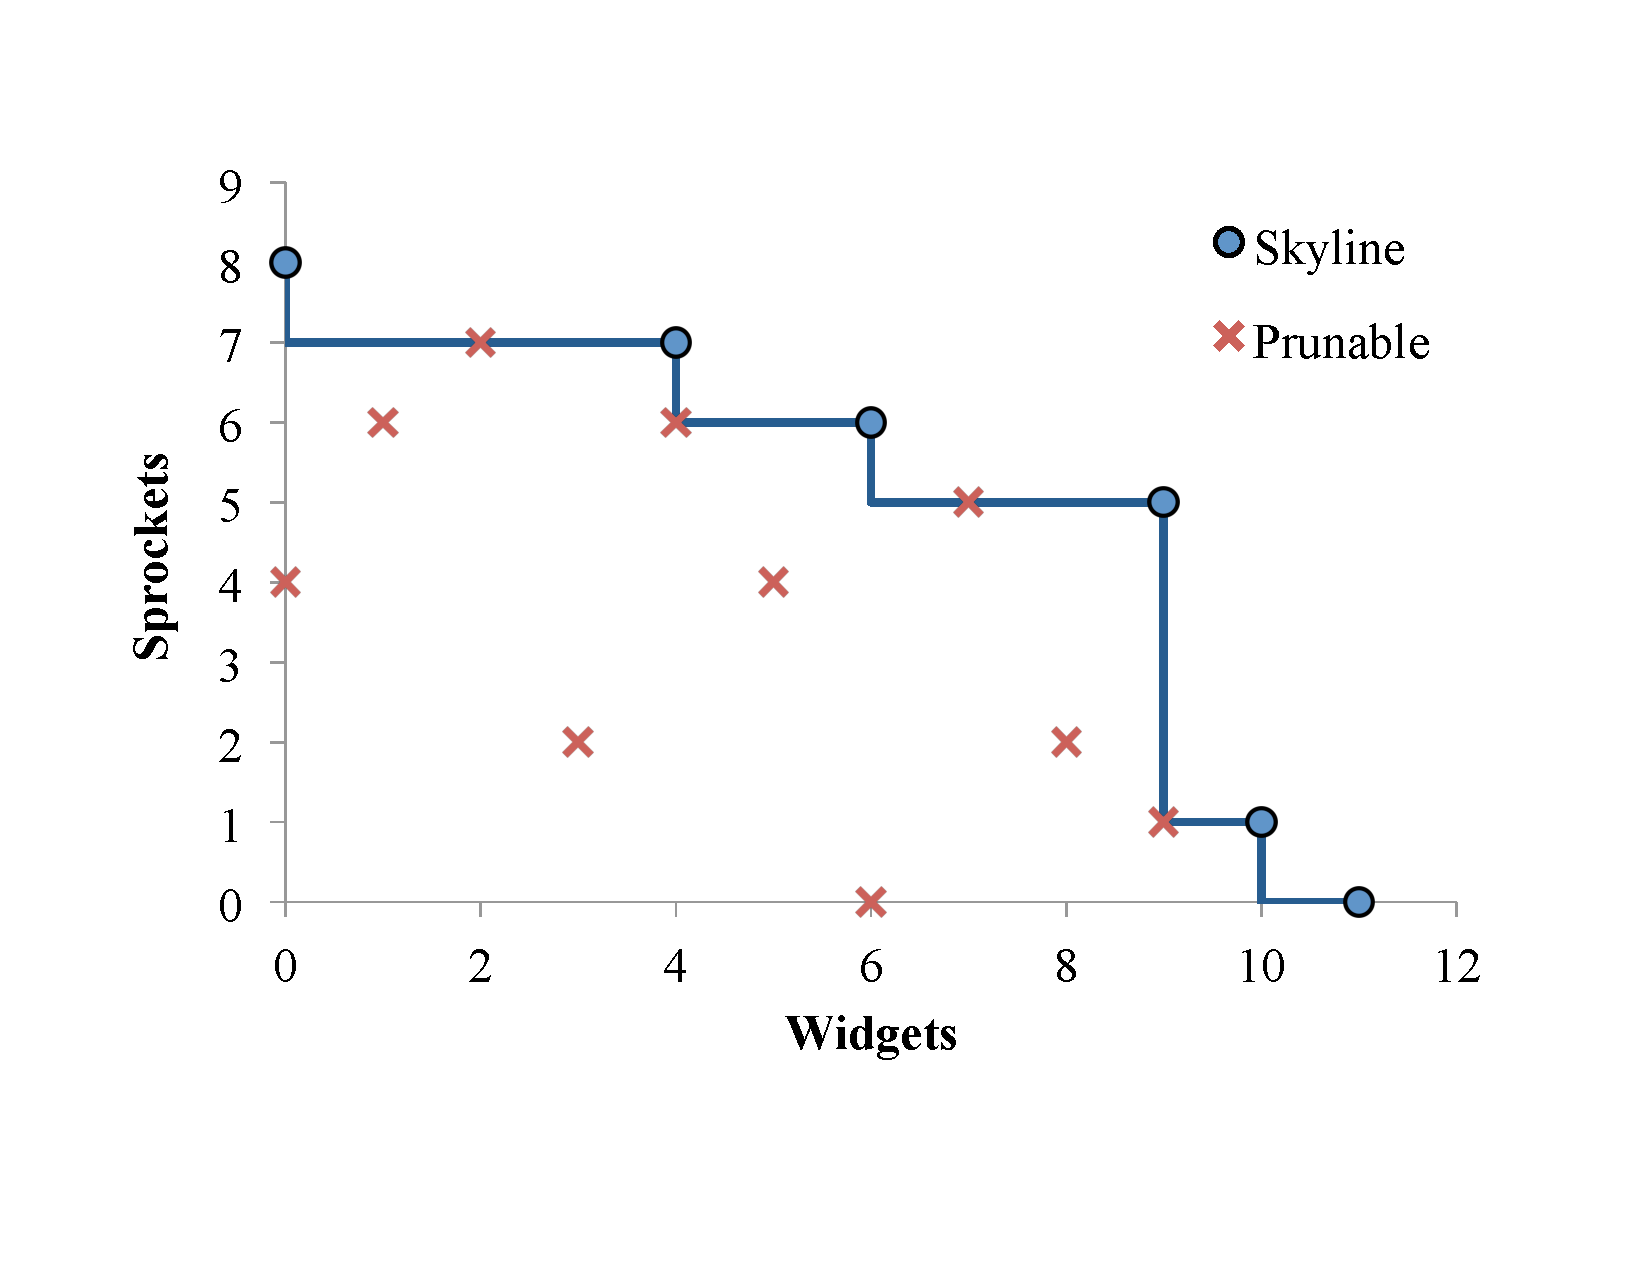
\includegraphics[width=3.3in]{skyline2d.pdf}
\end{center}
  \caption{An example set of states in a two-resource planning domain. If
all pictured states have the same cost, then only those shown as circles are
worth exploring; the X's can be safely pruned.}
  \label{fig:skyline}
\end{figure}


\subsection{Partial Orders}

We will further assume that our graph is endowed with a partial
order $\preceq$ that relates states $n$ to one another, with the
intuitive semantics that $n \preceq m$ if $n$ is no better than $m$
in any way. For example, in our sprockets and widgets example, $n
\preceq m$ if $n$ has no more widgets and no more sprockets than
$m$ and if $g(n) \ge g(m)$. Strict dominance $n \prec m$ holds if
$m$ is in addition strictly better than $n$ in some way.  For any
set of states $N$, we define the skyline of that set as
$\textrm{skyline}(N)=\{n: \not\exists n^\prime \in N: n \prec
n^\prime\}$. 

For example, in Figure \ref{fig:skyline}, we consider a domain with
two resources, widgets and sprockets. If having more widgets and
more sprockets is alway better, than all states that are not at one
of the corners of the skyline are strictly dominated by one or more
of the states that are.  Thus, if all states have the same cost,
we can safely remove those states from search.

Our goal is to define an optimal search algorithm that can exploit
this partial order to reduce the search space by only expanding
states $n$ that are \textit{weakly Pareto optimal}. That is, we
wish to only expand those states that are on the skyline. In the
next section, we will define this algorithm, and in the subsequent
sections, we will give a useful sufficient condition under which
we can exploit a partial order while preserving correctness of
optimal graph search algorithms.

We are not the first to suggest the use of Pareto optimality or
skyline queries in the context of planning. For example, the
non-optimal Metric-FF planner~\citep{hoffmann2003metric} employed
a more limited notion of dominance, requiring that all propositions
be the same between two states, the domain to be monotonically
``good'' in all resources, and for the dominating state to have no
fewer resources along any axis. Our notion of dominance is more
general. That is, we are able to find more powerful partial orders
in more general domains.

In another satisficing planner, \citet{roger2010more} combined
multiple heuristics by only expanding those states which were
currently Pareto optimal with respect to the current open set.  By
contrast, we seek to \textit{prune} search states while still
maintaining optimality.

Still others have employed fairly different notions of partial
orders while maintaining completeness and optimality. These methods
largely fall into a category known as ``partial order reduction
techniques,'' which have their origins in computer aided verification.
This class includes expansion cores \citep{chen09completeness,
xu11theory}, which select only ``relevant'' actions for any given
state, commutativity pruning~\citep{geffner2000admissible}, which
prunes redundant permutations of partial plans, and stratified
planning~\citep{chen2009stratified}, which identifies layers of the
planning problem and only considers actions appropriate to a given
layer. \citet{wehrle2012partial} recently showed that all of these
techniques are special cases of more general techniques from computer
aided verification, namely sleep sets~\citep{godefroid96partial}
and stubborn sets~\citep{valmari92stubborn}. These methods are
largely orthogonal to our approach; indeed, we use something not
unlike expansion cores in our system.


\subsection{Algorithm}

Skyplan is a fairly straightforward modification of a standard
optimal search algorithm like Uniform Cost Search or \Astar. For
the sake of exposition, we focus on Uniform Cost Search, though
\Astar or any optimal graph search algorithm can be modified in the
same way.\footnote{In our experiments we use either \Astar or
Hierarchical \Astar.~\citep{holte1996hierarchical}}

Skyplan is defined in Algorithm \ref{alg:skyplan}. Essentially, we
run Uniform Cost Search as normal, except that we only expand states
that are not strictly dominated by another state that we have either
expanded or enqueued for expansion. That is, we only expand nodes
that are in the \textit{skyline} of the nodes we know about so far.

Depending on the successor function, one might also want to compute
the skyline of the successors of the state being expanded and only
attempt to enqueue those nodes.  This check is purely an optimization,
not affecting optimality or completeness. Whether or not it is
useful depends on the kinds of search operators being applied: if
there are many similar successors to a state, this check can prune a very large
number of states. However, if most actions are very different, it will
likely have no effect.

\begin{algorithm}
  \begin{algorithmic}[1]
    \Procedure{UCSSkyplan}{$s, G, F, \preceq$}
    \State Initialize $Open=\{\langle s,0\rangle\}$, $Closed=\{\}$, $Pruned=\{\}$
    \While{ $Open$ is not empty}
    \State Pop the minimum cost state $\mathbf{n} = \langle n,c\rangle\in Open$
      \State $n\rightarrow Closed$
      \If {$n\in F$} 
        \State \Return the path to $n$ following back pointers
      \EndIf
      \If {$\forall m \in Open \cup Closed. n^\prime \nprec m$}
        \For {$n^\prime\in\mathrm{succ}(n)$} 
        \State $\mathbf{n^\prime} \gets \langle n^\prime,c+\mathrm{cost}(n,n^\prime)\rangle$
          \State $\mathbf{n^\prime} \rightarrow Open$
        \EndFor
      \EndIf
    \EndWhile
    \State fail
  \EndProcedure
  \end{algorithmic}
\caption{An implementation of Skyplan based on uniform cost search.  }
\label{alg:skyplan}
\end{algorithm}

\subsection{Compatibility}
\begin{figure}
	\begin{center}
	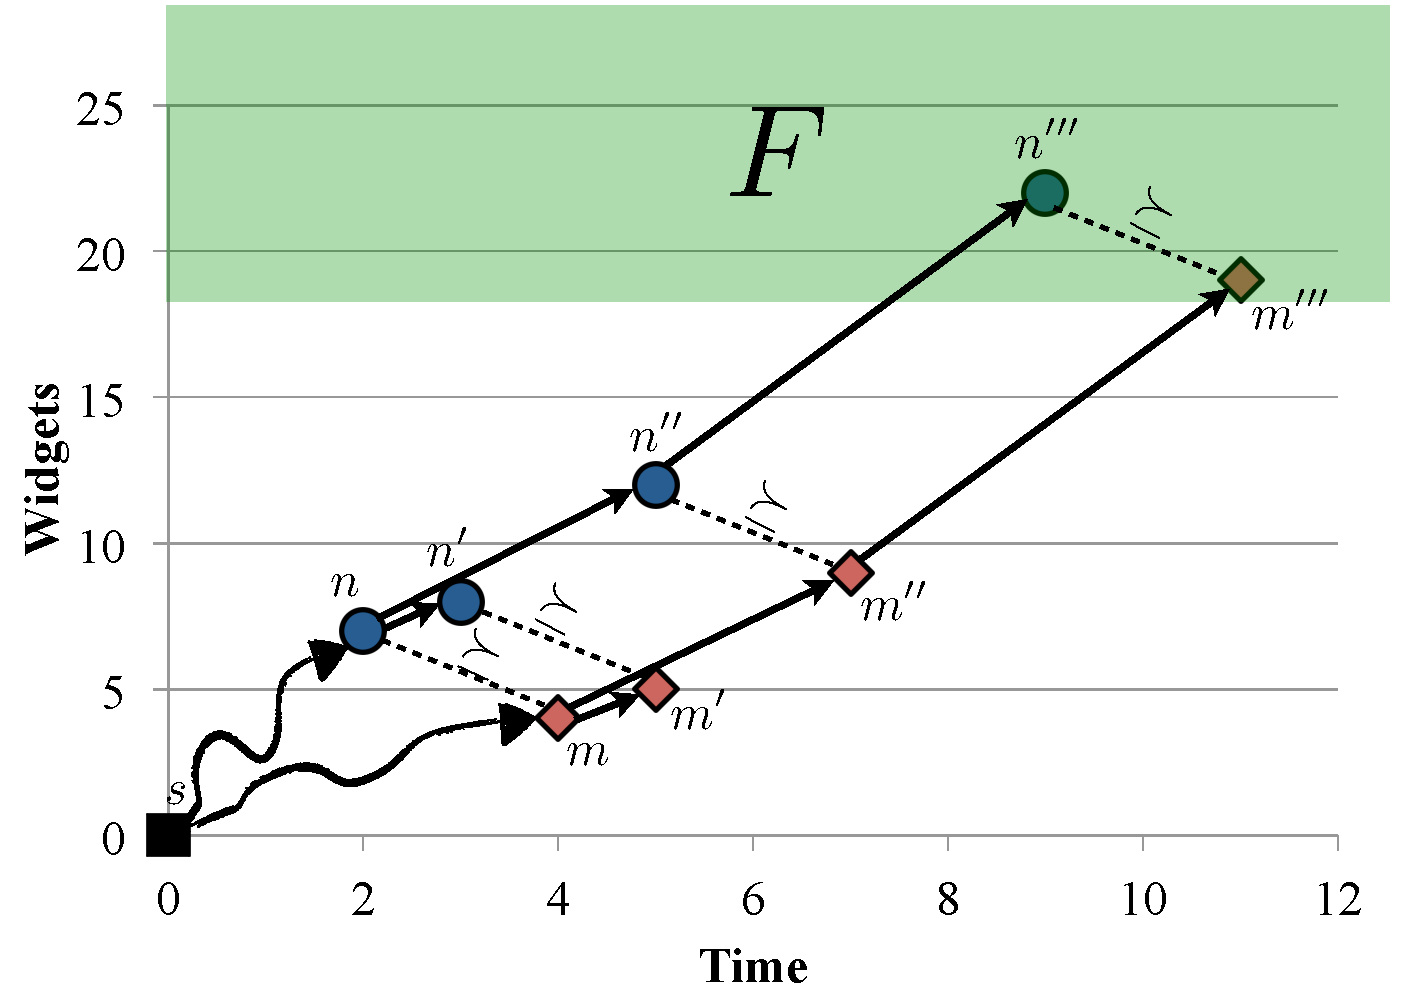
\includegraphics[width=3.3in]{compatibility-2.pdf}
\end{center}
  \vspace{-.2in}
  \caption{Abstract representation of search with compatible partial
  orders. Both $m$ and $n$ are reachable from the start state.
  Because $m$ is a better state than $n$, and $m$'s successors
  ``stay ahead'' of $n$'s, we can safely avoid expanding $n$ while
  still preserving optimality.}
  \label{fig:compatibility}
\end{figure}

Not just any partial order on states can be used to preserve optimality. As a perverse
example, we can define a partial order under which all states on the optimal path
are dominated by non-optimal states. Thus, we need to define a property
under which a partial order is \textit{compatible} with a search graph. While
a broad class of partial orders might work, we have identified a particular 
property that is especially applicable to planning problems:

\begin{definition}[Compatibility]
	\label{def-compatibility}
  A partial order $\prec$ is \textit{compatible} if for all states $m \preceq n$,
  \begin{enumerate}
    \item $g(n) \le g(m)$, and 
    \item $\forall m^\prime \in \mathrm{succ(m)}$ $\exists n^\prime \in
      \mathrm{succ}(n^\prime)$ such that $m^\prime \preceq n^\prime$ and
      $\mathrm{cost}(m,m^\prime) \ge \mathrm{cost}(n, n^\prime)$, and
    \item If $m \in F$, then $n \in F$
  \end{enumerate}
\end{definition}
This recursive definition of compatibility essentially means that
if a state $n$ is dominated by a state $m$, then it must be the
case that $n$ is no cheaper than $m$ and that $m$'s successors
``stay ahead'' of $n$'s. Finally, $F$ must be closed with respect
to $\succeq$: every state that dominates a goal state must also be
a goal. It is worth mentioning that there is always a compatible
partial ordering: the trivial order with $m \npreceq n$ for all
states $m$ and $n$.

Figure \ref{fig:compatibility} illustrates 
compatibility for a simple graph. If our goal is accumulate at
least 18 widgets, then $m$ is clearly better than $n$ as
it has more widgets in less time. Moreover, none
of $n$'s successors reach a point better than all of $m$'s 
successors. Because paths through $m$ continue to
``stay ahead'' of those passing through $n$, we
can safely prune $n$.

In planning problems, defining a compatible partial order is usually
quite easy, so long as cost functions are additive.  Actions are
often defined in terms of partial states with constant costs (e.g.\
time elapsed), and so compatibility is easily checked.  After proving
the correctness and optimality of Skyplan, we discuss a standard
structure for these partial orders, as well as how to automatically
infer a compatible partial order from the specification of a planning problem.

\subsection{Analysis}

In this section, we show that Skyplan is complete, optimal, and
optimally efficient for any compatible partial order when used in
conjunction with an optimal search algorithm like Uniform Cost
Search or \Astar. Before proving the main results of this section,
we prove a useful lemma.

\begin{lemma}{}\label{clm-complete-lemma}
  Let $p$ be a path to a goal, let $m$ be one state in $p$, and let 
$p_{n:}$ be the suffix of the path starting from $n$, and $|p|$
be
the length of a path in terms of the number of states. If $m$ is a state
with $m \succeq n$, then there is a corresponding path $q$ that reaches a goal state
through $n$ with $|q_{n:}| \leq |p_{m:}|$ and $\mathrm{cost}(q) \leq \mathrm{cost}(p)$.
\end{lemma}

\begin{proof}
$p_{m:}=(m,m_{1},\dots,m_{k})$ with $m_{k}$ a goal state.
By condition (2) of compatibility, $\exists n_{1} \in \mathrm{succ}(n)$ 
with $n_{1} \succeq m_{1}$ and $\mathrm{cost}(n,n_{1}) \leq \mathrm{cost}(m,m_{1})$. 
Similarly, $\exists n_{2},\dots,n_{k}$ with 
$n_{i} \succeq m_{i}$ and $n_{i+1} \in \mathrm{succ}(n_{i})$ with 
total cost $\leq \mathrm{cost}(p_{m:})$.
By condition (3) of compatibility, $n_{k} \in F$. By condition (1),
there is a path from $s$ to $n$ with $g(n) \leq g(m)$. The above argument extends this path
to the goal state $n_{k}$ and completes the proof of the lemma.
\end{proof}

This lemma states that if $m \preceq n$, then there is a path from $n$ to a goal
state that is no longer and no more costly than any such path from $m$.
While we usually consider states being pruned by other states, the lemma
allows us to equivalently reason about paths being pruned by other paths.
In the following proof, we use these notions interchangeably.


\begin{claim}{Completeness.}\label{clm-complete}
   If $\preceq$ is a compatible partial order, Skyplan
is \emph{complete}.
\end{claim}
\begin{proof}
Suppose otherwise, then all paths to all goals must
have been pruned. This would require a cycle of paths pruning each other: 
paths $p^{1},\dots,p^{k}$ such that $p^{i+1}$ was pruned by $p^{i}$ (letting $p^{0}=p^{k}$) .
For all paths, let $n_{i+1} \in p^{i+1}$ be the state which pruned $p^{i}$ and
$m_{i} \in p^{i}$ the corresponding state which was pruned 
($\forall i: m_{i} \preceq n_{i+1}$).

Because each $m_{i}$ was pruned before being expanded,
$n_{i} \neq m_{i}$ nor any state succeeding $m_{i}$ in $p^{i}_{m_{i}:}$.
Hence $p^{i}_{n_{i}:} \supsetneq p^{i}_{m_{i}:} \implies |p^{i}_{n_{i}:}| > |p^{i}_{m_{i}:}|$.
By the lemma, we also have % \reference?
 $|p^{i}_{m_{i}:}| \geq |p^{i+1}_{n_{i+1}:}|$. Combining the
inequalities yields: $|p^{1}_{m_{1}:}| \geq |p^{2}_{n_{2}:}| > |p^{2}_{m_{2}:}| > \dots > |p^{k}_{m_{k}:}| > |p^{1}_{m_{1}:}|$, 
a contradiction.
\end{proof}
  
\begin{claim}{Optimality.}\label{clm-optimal}
   If $\preceq$ is a compatible partial order, Skyplan
is \emph{optimal}.
\end{claim}
\begin{proof} 
Let $p^{*}$ be the last optimal path that was pruned during a run of Skyplan. 
By the proof of Claim \ref{clm-complete} and the lemma 
there is some path $p^\prime$ that is not pruned with
$\mathrm{cost}(p^\prime) \leq \mathrm{cost}(p^{*})$.
Thus, $p^\prime$ is optimal as well.
\end{proof}

By leveraging the information contained in the partial order, Skyplan is able to achieve
optimal plans while expanding fewer states in general.  But is Skyplan using this added
information in the best possible manner? It is easy to see that any state expanded by 
Skyplan must not be dominated by any other state in the graph: otherwise $Closed$ would
contain such a dominating state when the about-to-be-expanded
state was popped, thereby pruning it.  This turns out to be
enough to prove the following:

\begin{claim}{Optimal Efficiency.}\label{clm-optimally-efficient}
For any compatible partial order $\prec$, Skyplan is \emph{optimally efficient}.
\end{claim}
\begin{proof} 
(We prove the claim on the set of graphs for which all paths have unique costs: $n \neq m \implies g(n) \neq g(m)$.)

Suppose otherwise. Then, there must exist an optimal algorithm B and a search problem $(G,\preceq)$ 
on which B expands (calls the successor function on) strictly fewer states than Skyplan. 
Let $n^{*}$ be a state expanded in Skyplan but not by B on the problem $(G,\preceq)$, and let
$f_{B}$ be the goal state returned by B. We construct a new graph $G^\prime$ by adding a single goal state $f^*$ to $G$ 
and an associated edge from $n^*$ to $f^*$ of cost $\epsilon$ (with $\epsilon < g(f^*)-g(n^*)$). 
On $G^\prime$ we apply the original partial order $\preceq$ with $n \npreceq m$ if either $n$ or $m$ is $f^*$.

We must show that $\preceq$ is compatible on $G^\prime$. 
Let $m,n \in G^\prime$ such that $n \preceq m$. Then neither $m$ or $n$ is $f^*$. Conditions (1) and (3) %\ref
are clearly true in $G^\prime$ because they are true in $G$.  Furthermore, if $n \neq n^*$ condition (2) is true 
because $succ_{G^\prime}(n) = succ_{G}(n)$. 
But as we observed above, no state expanded in Skyplan is dominated by any other state $\implies n \neq n^*$.

Except for the fact that $n^*$ has an extra successor, $G^\prime$ is otherwise
 identical to $G$. By assumption, B never examined the successors of $n^*$, and 
must therefore follow the same execution path on the graph $G^\prime$, returning the goal state $f_B$.
But by construction, $f^*$ is a lower-cost goal in $G^\prime$, contradicting the optimality of B.
 \end{proof}


\section{Inferring Partial Orders}

\newcommand{\po}{\preceq_R}

Now that we have a definition of compatible partial orders and an
algorithm that can take advantage of them, all we need is a method
for finding them. Of course, one can construct them by hand using
domain knowledge, but that is less than ideal. In this section, we
show how to automatically infer a compatible partial order from a
sequential planning problem domain's specification, such as those
available in PDDL.~\citep{ghallab1998pddl,fox2003pddl2} In the next
section, we will extend this procedure to a broad class of concurrent
domains with durative actions.

\subsection{Planning States}

When planning with resources, a basic planning state $n$ can be viewed as a mapping from
resource types to values. That is, for a given resource $r$, $n(r) \in \R$ is the quantity
of that resource available at state $n$. Most planning state representations also require
some notion of boolean propositions, but in order to simplify the exposition, for the
purposes of defining a partial order we view these as special resources that always take
values in \{0, 1\}.

Also note that for planning problems, the \emph{cost} of a state is
just a resource like any other. For example, in many domains, the cost is equivalent to
time, which most actions increment as one of their effects. Thus, though we have been so
far using $g(n)$ to refer to the cost of the \emph{optimal} path to a state, in this
section we will abuse notation slightly and treat $g(n)$ as an observable property of the
state itself, with the understanding that a path with a different cost would have reached a
different state.

\subsection{Basic Partial Orders}

If we want to determine whether a state $n$ dominates $m$, then we need
to know two things: first, does $n$ have lower cost; and second, does $n$
have a more ``useful'' set of resources? The first criterion is easy to check, but the
second requires some notion of what it means for a resource to be useful or not.

There are basically two ways in which the value of a particular resource can matter: it can
either contribute to satisfying the goal test $n \in F$, or it can contribute to satisfying
the precondition of some action that might get us closer to the
goal. In both cases, we are
concerned with the relationship between the value of a particular resource $r$, and a
particular boolean predicate $b$. In general, we want to know when it helps to have more (or less) of a particular resource, leading us to the following classification
of predicates based on how they interact with a given resource. Let $b(n)$ be the value of the predicate $b$ in state $n$.
\begin{definition}[$r$-Dependent]
A predicate $b$ is $r$-\textit{dependent} if $\exists n, n^\prime$ with $b(n) = \text{true}$ and $b(n^\prime) = \text{false}$, but where $n$ and $n^\prime$ are identical except that $n(r) \ne n^\prime(r)$.
\end{definition}
\begin{definition}[$r$-Positive]
	A predicate $b$ is $r$-\textit{positive} if $b$ is $r$-dependent and
	\begin{enumerate}
		\item $\forall n, n^\prime$ identical except $n(r) < n^\prime(r)$, $b(n) \Rightarrow b(n^\prime).$
		\item $\forall n, n^\prime$ identical except $n(r) > n^\prime(r)$, $\neg b(n) \Rightarrow \neg b(n^\prime)$
	\end{enumerate}
\end{definition}
\begin{definition}[$r$-Negative]
	A predicate $b$ is $r$-\textit{negative} if $b$ is $r$-dependent and
	\begin{enumerate}
		\item $\forall n, n^\prime$ identical except $n(r) > n^\prime(r)$, $b(n) \Rightarrow b(n^\prime).$
		\item $\forall n, n^\prime$ identical except $n(r) < n^\prime(r)$, $\neg b(n) \Rightarrow \neg b(n^\prime)$
	\end{enumerate}
\end{definition}
For example, the predicate ``$n(r) \ge 1$'' is $r$-positive, the predicate ``$n(r) \le 0$'' is \textit{r-negative}, the predicate ``$n(r_1) \ge n(r_2)$'' is $r_1$-positive, but $r_2$-negative, and the predicate ``$1 \le n(r) \le 2$'' is $r$-dependent, but neither $r$-positive nor $r$-negative.

Using these definitions, we can construct a partial order based on three parts of the problem definition:
\begin{enumerate}
	\item The set of (grounded, where applicable) resources.
	\item The set of possible (grounded) actions, particularly their preconditions.
	\item The goal test: $n \in F$.
\end{enumerate}

Let $B$ be the set of all relevant predicates, that is, the set of preconditions for each action plus the goal test. Then we partition all the resources into four disjoint sets: $R^+$, $R^-$, $R^=$, and $R^\emptyset$, according to the following criteria:
\begin{itemize}
	\item $r \in R^+$ if $\forall b \in B, b$ is $r$-dependent implies that $b$ is $r$-positive, and $\exists$ at least one $b \in B$ that is $r$-positive.
	\item $r \in R^-$ if $\forall b \in B, b$ is $r$-dependent implies that $b$ is $r$-negative, and $\exists$ at least one $b \in B$ that is $r$-negative.
	\item $r \in R^=$ if $\exists b \in B$ that is $r$-dependent but not $r$-positive or $r$-negative, \emph{or} if $\exists b_1, b_2 \in B$ with $b_1$ $r$-positive and $b_2$ $r$-negative.
	\item $r \in R^\emptyset$ if $\forall b \in B, b$ is \emph{not} $r$-dependent.
\end{itemize}

These sets are fairly intuitive. For instance, resources in
$R^+$ are better the more you have of them (e.g.\ widgets),
while resources in $R^=$ have a complex relationship with
the problem, and so it is not safe to prune a state $n$ unless
it has the exact same value as its potential dominator for that
resource.  $R^\emptyset$ consists of those resources that
have no effect on any condition in the problem. Finally, we can define the partial order $\po$:

\begin{definition}[$\po$]
	\label{def-po}
	For planning states $n$ and $m$, we say that $n \po m$ if and only if:
	\begin{enumerate}
		\item $g(n) \ge g(m)$,
		\item $\forall r \in R^+, n(r) \le m(r)$,
		\item $\forall r \in R^-, n(r) \ge m(r)$, and
		\item $\forall r \in R^=, n(r) = m(r)$
	\end{enumerate}
\end{definition}

\begin{claim}{}{\label{clm-po-compatible}}
	If action costs and effects do not depend on the current state, then $\po$ is compatible.
\end{claim}
\begin{proof}
	Condition 1 of Definition~\ref{def-compatibility} follows directly from condition 1 of Definition~\ref{def-po}.
	
	To verify condition 3 of Definition~\ref{def-compatibility},
  we only need to consider resources $r$ for which the goal
  test is $r$-dependents, as changes in other resources will not affect the outcome of the test. If the goal test is $r$-positive, then $r \in R^+$ or $r \in R^=$, so $n(r) \le m(r)$. If the goal test is $r$-negative, then $r \in R^-$ or $r \in R^=$, so $n(r) \ge m(r)$. If the goal test is neither (but is $r$-dependent), then $r \in R^=$, so $n(r) = m(r)$. Taken together, these conditions ensure that $n \in F \Rightarrow m \in F$.
	
	Finally, to verify condition 2 of Definition~\ref{def-compatibility}, observe that some particular action results in the transition from $n$ to $n^\prime$. By the argument above, if the precondition of this action holds for $n$, then it also holds for $m$. Let
  $m^\prime$ be the result of taking this action from $m$. By assumption, the cost is identical, and also by assumption, the change in resources from $m$ to $m^\prime$ is identical to that from $n$ to $n^\prime$, which implies that $\forall r, m^\prime(r) -
  n^\prime(r) = m(r) - n(r)$. Therefore, $n^\prime \po m^\prime$.
\end{proof}

A few remarks are in order with regard to this inferred ordering.
First, it may not be the best ordering for a given problem. Consider a domain in
which we need can use sprockets to make a transmogrifier, but
not widgets. However, suppose there is a free conversion from widgets
to sprockets, and vice versa---because sprockets are in fact just
upside down widgets. In this case, sprockets and widgets are
interchangeable, and so we can actually prune based on the sum of
their count. However, this method is incapable of realizing this
relationship. In general we suspect that it is
intractable to find the
optimal partial ordering, but that such perverse examples
as the one just described are rare.

Second, there are occasionally resources that are usually beneficial,
but they might have some high upper limit. For instance, we might
like to have as many widgets as possible, except that we have only
a large but finite amount of storage space for them.  In this case,
we would not be able to prune based on the number of widgets: its
resource would be in $R^=$. However, if the maximum number of widgets
is indeed so high that we suspect that we will not reach it in
search, we can treat it as though there was no limit. If we do in
fact hit the limit, we then have to re-enqueue all nodes pruned
based on widget count, and back off to the safer partial order.

\section{Partial Orders and Concurrency} 

In classical planning domains, constructing a search graph is
straightforward, with transitions corresponding directly to the
simple actions available to the agent. However, in planning domains
that permit multiple simultaneous actions, the state space and the
search graph need to be augmented slightly for planning to still
work properly as a search problem. In this work, we use a mild
adaptation of the concurrent planning framework described in
\citet{bacchus2001planning}.
First, we briefly describe this representation, and then describe
the extension of the partial order inference to concurrent domains.

\subsection{Modeling Concurrency}

The main modification is that each action no longer necessarily
makes only atomic modifications to a state. Instead, action effects
now have three parts: effects that take place immediately upon
beginning the action, the duration required before the action
completes, and effects that take place when the action ends. In
order to keep track of actions whose completion effects haven't
occurred yet, basic states are augmented with an \emph{action queue}.
An action queue is a multiset of $(a, t)$ pairs, where $a$ is an
in-progress action, and $t$ is the length of time until that action
completes.

The search graph also needs to be modified to handle in-progress actions. First, 
in this work, we assume that the cost function used in concurrent planning domains is
$C_a + \lambda T$, where $C_a$ is the accumulated cost of all basic actions taken, $T$ is
the total amount of time elapsed, and $\lambda > 0$ is a scaling constant. The search graph still contains transitions for all
basic actions whose preconditions are satisfied, each with the same cost. However, the
construction of the ending state $n^\prime$ is different: when performing action $a$, only the
\emph{immediate} effects are applied, and then the pair $(a, d_a)$ is added to the action
queue, where $d_a$ is the duration of $a$. 
In addition to the transitions for basic actions, we also need a set of special transitions
$\mathrm{elapse\_time}(k)$. The cost of this transition is $\lambda k$, and the effects are: 
\begin{enumerate}
	\item For every pair $(a, t)$ on the action queue with $t \le k$, the \emph{completion} effects of $a$ are applied.
	\item All pairs $(a, t)$ with $t \le k$ are removed from the action queue.
	\item All pairs $(a, t)$ with $t > k$ are replaced with $(a, t-k)$.
\end{enumerate}


\subsection{Inferring Partial Orders with Action Queues}

\newcommand{\poq}{\preceq_Q}

In concurrent domains, in addition to a collection of resources, the state contains a queue
of in-progress actions. Here, we'll construct a new partial order $\poq$ that takes the
action queue into account. To simplify the exposition, we assume that all
actions have \emph{beneficial} completion effects.\footnote{This assumption is met in all
domains we consider in this work.} Formally, this means that any resource whose value is
increased at completion is in $R^+$ or $R^\emptyset$, and any resource whose value is decreased is in
$R^-$ or $R^\emptyset$. The extension to more general action effects is straightforward.

Intuitively, a state $m$ can only be better than a state $n$ if
its action queue finishes faster than $n$'s, or if $m$ already
has more resources than $n$ will have. We formalize this
intuition as follows:

\begin{definition}[$\poq$]
	\label{def-poq}
	Let $q(n)$ denote the action queue for state $n$. For planning states $n$ and $m$, we say that $n \poq m$ if and only if $n \po m$, and $\forall (a, t) \in q(n)$, at least one of the following conditions holds:
	\begin{enumerate}
		\item $\exists$ a distinct $ (a, t^\prime) \in q(m)$ with $t^\prime \le t$.
		\item $\forall r $ affected by the completion effects of $
      a$, the change from $n(r)$ to $m(r)$ is at least as big
      as that produced by all actions currently enqueued that
      are not satisfied by condition 1.
	\end{enumerate}
\end{definition}
The notion of a \emph{distinct} pair $(a, t^\prime)$ is important, as the same action can appear multiple times in the same action queue. For example, let $a$ be an action whose completion effect is ``Gain 5 $r$''. If $q(n) = \{(a, 10), (a, 20)\}$ then $q(m) = \{(a, 10),
(a, 15)\}$ meets this condition, but $q(m) = \{(a, 5)\}$ does not, unless $m(r) \ge n(r) + 5$. Similarly, $q(m) = \{\}$ does not meet the condition unless $m(r) \ge n(r) + 10$.

\begin{claim}{}{\label{clm-poq-compatible}}
	If action costs and effects do not depend on the state, and all action completion effects are beneficial, then $\poq$ is compatible.
\end{claim}
\begin{proof}

	The proof of Claim~\ref{clm-po-compatible} already covers conditions 1 and 3 of
Definition~\ref{def-compatibility}. There are two types of transitions we need to handle
for condition 2: basic action transitions, and $\mathrm{elapse\_time}$ transitions. Basic
actions are also mostly covered by the proof of Claim~\ref{clm-po-compatible}; the only
difference is that the action queues are modified. $q(n)$ and $q(n^\prime)$ differ only in
the addition of $(a, d_a)$, and likewise for $q(m)$ and $q(m^\prime)$. This new addition is
covered by the first case in Definition~\ref{def-poq}, and $n \poq m$ implies that the rest
of $q(n^\prime)$ is matched by $m^\prime$, so we also have $n^\prime \poq m^\prime$.

	All that remains is the $\mathrm{elapse\_time}$ transitions. Assume that $n^\prime$ is
reached by following $\mathrm{elapse\_time}(k)$ from $n$. If we follow $\mathrm{elapse\_time}(k)$ from $m$, we incur the same cost and $m^\prime$ has the following two properties. First, for every pair $(a, t) \in q(n)$ with $t \le k$ that is completed as part of the transition, either:
\begin{enumerate}
	\item $m$ already had a corresponding resource advantage over $n$ and thus $n^\prime$ does not overtake $m^\prime$, or
	\item $\exists (a, t^\prime) \in q(m)$ with $t^\prime \le t \le k$, and so this action completes and $m^\prime$ gets a corresponding resource improvement.
\end{enumerate}
Second, for every pair $(a, t) \in q(n)$ with $t > k$ there is now a pair $(a, t-k)$ in $q(n^\prime)$. But in $m^\prime$, one of three conditions holds:
\begin{enumerate}
	\item $m$ already had a corresponding resource advantage over $n$, so $m^\prime$ preserves this advantage over $n^\prime$, or
	\item $\exists (a, t^\prime) \in q(m)$ with $k < t^\prime \le t$, so $(a, t^\prime-k)$ is in $q(m^\prime)$, or
	\item $\exists (a, t^\prime) \in q(m)$ with $t^\prime \le k \le t$, so $m^\prime$ has gained the necessary resource advantage over $n^\prime$.
\end{enumerate}
Taken altogether, we once again get $n^\prime \poq m^\prime$.

\end{proof}

\section{Skyplan in Practice}

Thus, the basic outline of our system is fairly straightforward.
Given a planning problem, Skyplan infers the partial order
and we then use that partial order in a standard graph search.

There are a few pragmatic details of our system that can substantially
affect performance that are worth mentioning. One is our choice of
Hierarchical \Astar~\citep{holte1996hierarchical} as base search
algorithm, since we found to be one of the best algorithms. The
other is the somewhat more mundane question of how best to implement
a skyline query for our setting.  In this section, we discuss each
in turn.

\subsection{Hierarchical \Astar}

While skyline pruning works with any optimal search procedure, this
pruning method has a particular synergy with the Hierarchical \Astar
algorithm. Hierarchical \Astar works
by identifying a series of relaxations to the search space, and
uses each level of relaxation as the (admissible and consistent)
heuristic for the corresponding lower level.

One particularly easy way to apply this algorithm to planning is
to define the relaxations only in terms of relaxations to the goal
test. That is, one can simply take a subset of the goal conditions
at each level without any further relaxations of the state space. 

If we use this series of projections, we can actually maintain a
\textit{single} skyline for all levels of the hierarchy so long as
we use the partial order $\po$ defined on the original search problem
(that is, with the full goal test). Thus, when expanding a lower
level state, we can prune any of its successors if they are dominated
by a state at \textit{any} level of the hierarchy.  In particular,
the combination of Hierarchical \Astar and skyline pruning means
that the projected searches give us two sources of information: how
far a state is from a (partial) goal, and which states are not
possibly on the optimal path to the full goal. 

\subsection{Implementing Skyline Pruning}

The implementation of skyline pruning is somewhat delicate.  There
is some work in this area in the database literature, but these are
not designed for online applications~\citep{skylineoperator,tan01efficient}
or are for fairly low dimensional states~\citep{KossmannRR02}, and
so they are not useful here.

The obvious, na\"ive solution is to maintain a list of all elements
in the current the skyline, and to check all of these elements when
deciding whether or not to add an element to the skyline. Unfortunately,
this check is clearly linear in the number of states (which means
we must make quadratically many checks), In practice, this
runtime can overwhelm the benefit obtained from pruning the branching factor.

However, note that in high dimensions most states are clearly not
related to one another.  They might both have different positive
propositions, with one not having strictly more than another.
Therefore, we can quickly do a ``coarse'' version of a skyline query
by having a list of sets, one for each resource or proposition,
that contains all states in the skyline that have a positive value
for that resource if the resource is in $R^+$, and
vice versa if negative. Then, when deciding whether or not a new
state is dominated, we can simple intersect these sets, and then
run the check on those states in the intersection. Because most
states in practice are dominated by very few (or sometimes no)
states, this intersection is much smaller than the entire skyline.
So, while this optimization does not decrease the asymptotic runtime,
in practice it is several orders of magnitude faster.



\section{Experiments}

We empirically evaluated Skyplan in two domains. First, we ran experiments on a collection
of standard job shop tasks from the woodworking domain. We chose this domain because it
permits simultaneous actions, and Skyplan is particularly well-suited to domains where the
extra freedom afforded by concurrency results in an explosion in the set of possible
states. However, like most standard planning domains, this one is largely concerned with
discrete objects rather than ever-growing resources, and so is still rather limited in the
amount of concurrency needed, with even the most complex problems never permitting more
than a dozen simultaneous actions, and the simpler problems that were amenable to optimal
planning not requiring more than 2. Thus, we also ran experiments in a more realistic
resource acquisition setting modeled on the video game StarCraft.

\subsection{The Woodworking Domain}

We used the woodworking problems released with 2008
International Planning Competition.
Though the later problems are fairly challenging and require satisficing solutions,
the earlier problems are simple enough to be solved by basic optimal planners. We compare
Skyplan to basic Hierarchical \Astar on the first 5 problems from this domain. We measured
the number of nodes popped (including those popped during the recursive searches used
for heuristic computation) and the total time taken by each algorithm.\footnote{All
these experiments were run on isolated 2.67GHz Intel Xeon processors.} The results are
shown in Table~\ref{tab:woodworking}.

\begin{table*}
	\begin{center}
		\begin{tabular}{|c|cc|cc|cc|cc|cc|}
		\hline
		\multirow{2}{*}{Planner} & \multicolumn{2}{c|}{Problem 1}  & \multicolumn{2}{c|}{Problem 2} & \multicolumn{2}{c|}{Problem 3} & \multicolumn{2}{c|}{Problem 4} & \multicolumn{2}{c|}{Problem 5} \\
		& Nodes & Time & Nodes & Time & Nodes & Time & Nodes & Time & Nodes & Time \\
		\hline
		Hierarchical \Astar & 732 & 0.148 & 4762 & 1.11 & 19,010 & 4.13 & 260,375 & 129 & 2,620,531 & 1515 \\
		Skyplan         & 442 & 0.096 & 2615 & 0.76 & 11,709 & 3.58 & 135,675 & ~99 & & \\
		\hline
		\end{tabular}
	\end{center}
	\label{tab:woodworking}
	\caption{Results on the woodworking domain. Times are in seconds, and are averaged over 20 runs for problems 1, 2, and 3; over 10 runs for problem 4; and over 5 runs for problem 5.}
\end{table*}

Skyplan is consistently faster than Hierarchical \Astar, typically pruning almost 50\% of the
nodes that H\Astar expands. Maintaining the skyline does impose some overhead cost, but Skyplan
still retains anywhere from a 15\% to a 35\% speed advantage.

\subsection{The StarCraft Domain}

StarCraft$^\textrm{\textregistered}$ is a real time strategy game
created by Blizzard Entertainment, and one of the most competitive
and popular games in the world. The game involves the accumulation
of resources (minerals and gas), which are gathered by workers.
These resources are then spent to build structures (e.g.\ a barracks),
which are then in turn used to build military units. The ultimate goal is
to build an army to defeat an opponent.


There are many aspects of this game that are worth modeling from
an artificial intelligence perspective in general and from planning
in particular. The game lends itself to partial observability,
planning against an adversary, highly concurrent plans, and online
planning.  Indeed, \citet{churchill11build} recently described an
online planning system designed for use in an artificial intelligence
agent, and \citet{chan07online} earlier developed an online planner
for a similar open source game called Wargus.

Here, we focus instead on planning opening build orders. Much like
Chess, there are a large number of different openings, some of which
are known to be better than others. In StarCraft, openings can be
either more aggressive or more ``economic'' (i.e.\ aimed at producing
lots of resources), and typically are designed to get a specific composition
of buildings and units as quickly as possible.  In practice, the
first several minutes of the game are played largely independent
of what the opponent is doing, unless certain surprise ``cheese''
openings are observed. Moreover, shaving seconds off an opening can
be the difference between an easy early win and a loss. Thus, coming
up with an optimal build order for a given composition is useful,
if it is feasible.

One crucial aspect of StarCraft is that workers are both the resource gatherers
and the builders of buildings. Combined with StarCraft being a ``real time'' game, 
this property results in an extremely high branching factor in the game tree. However,
many of the possible combinations are clearly not optimal: it is usually (but not always) a bad idea
to have your workers remain idle. This aspect of the game results in a large number of highly similar
states, most of which are worse than others.

Our specification of StarCraft differs from that of
\citet{churchill11build} precisely in how we handle gathering
resources. For simplicity, they assume a linearization of resource
gathering, with resources gathered at a continuous rate. However,
resources are actually gathered in discrete amounts. By more
accurately modeling resource collection, we can find more
accurate plans, particularly in the early game, where seconds
are so critical.\footnote{We will release a PDDL version
of this specification upon publication.}

\section{Conclusion}

Planning in highly concurrent domains can be particularly challenging for standard
search-based planners, but by restricting attention to only those states that could
conceivably be part of an optimal plan, Skyplan can efficiently solve problems that
previously could only be tackled by satisficing approaches. Furthermore, since
geometrically pruning the state space achieves speedups in a way that is orthogonal to
heuristic domain knowledge, this gain should stack well with improved A* approaches. There
is overhead introduced by the optimality-preserving skyline, but further innovations in
data structures for state space pruning could obviate this problem, perhaps trading
guaranteed optimality for improvements in asymptotic complexity.

\bibliographystyle{aaai}
\bibliography{refs}

\end{document}
